\documentclass[a4paper,12pt,twoside]{report}
\usepackage[left=3cm,right=3cm,top=2cm,bottom=3cm]{geometry}
%\usepackage[square,authoryear,sort]{natbib}
\usepackage{url}
\usepackage{xcolor}
\usepackage{graphicx}
\usepackage{pdfpages}
\usepackage{subcaption}
%\usepackage{pgfgantt}
\usepackage{dirtytalk}

\makeatletter
\def\@makechapterhead#1{%
  \vspace*{50\p@}%
  {\parindent \z@ \raggedright \normalfont
    \interlinepenalty\@M
    \Huge\bfseries  \thechapter.\quad #1\par\nobreak
    \vskip 40\p@
  }}
\makeatother

\makeatletter
\newcommand*{\toccontents}{\@starttoc{toc}}
\makeatother

\newtheorem{hypothesis}{Hypothesis}

\newtheorem{rquestion}{Research Question}


\let\endtitlepage\relax
\begin{document}

\title{\LARGE {\bf PhD Research Proposal:\\Semantic Modelling of Network Traffic for Anomaly Detection}\\
 \vspace*{-5mm}
}
\author{Henry Clausen}
%\date{October 2008}

\maketitle



\toccontents
%\begin{abstract}
%Text
%\end{abstract}



\chapter{Research description}

%\section{Introduction and motivation}

\section{Intrusion detection}

Sophisticated data breaches affect hundreds of million customers and inflicts tremendous financial, reputational, and logistic damage. One reason for the recent rise of cyber crime is the increased use of sophisticated techniques for the attack of specific targets. Attackers use customised social engineering and custom-build malware that penetrate defensive barriers and potentially stay undetected in an infected system for an extended period of time. 

Cyber-Security relies on a range of defensive techniques, including sophisticated intrusion detection systems and firewalls that try to detect and prevent attacks against software subsystems. Malicious software still remains the biggest threat to computer users, and its detection is of utmost importance. 

The field of intrusion detection is concerned with the development of methods and tools that identify and locate possible intrusions in a computer network. An \textit{intrusion detection system} (IDS) is typically a device or software application that detects malicious activity or policy violations in an automated way by scanning incoming data collected from one or more sources for patterns that a model or a set of rules classifies as malicious.

Intrusion detection is a well researched area, with the first IDSs emerging in the late 1980's. Intrusion detection today comprises a variety of research areas in terms of different types of data sources, system architectures, detection sope, and so forth. Denning \cite{denning1987intrusion} in 1987 established the notion of two different types IDS implementations: a) host-based and b) network-based. 
\textit{Host-based intrusion detection systems} (HIDS) monitor each host in a network individually, and rely on local data streams such as application logs or raw operating system calls as  data source. \textit{Network-based intrusion detection} refers to the detection of malicious traffic in a network of computers and uses network traffic captures as a data source. In this PhD project, I will mainly focus on network traffic as a data source due its universal nature, its resilience against modification, and my previous experience in the field. However, I will also investigate the possibility of relating both types of traffic. For more details on IDS implementations, I refer the reader to my more detailed literature review. 


Current detection methods are predominantly based on the analysis of previously identified attack signatures, which provides great reliability and low false alert rates. However, these methods are dependent on an updated attack signature database and provide no protection against previously unseen attacks. With attackers having access to more resources than ever, custom built malware is becoming more common to circumvent signature-based detection. 

Another approach that has recently gained traction in commercial deployment is based on detecting malware and other undesired activity as anomalous behaviour when compared to benign computer activity. In this approach, known as \textbf{network anomaly detection}, models that quantify the behaviour of normal network behaviour in order to be independent of a narrowly defined notion of malicious activity.



\section{Anomaly detection}

Anomaly detection refers to the problem of identifying data instances that have significantly different properties than previously observed \say{normal} data instances. Anomaly detection has its origins in statistical research where normal data instances are assumed to be generated as random variables by a probability distribution $P_\textit{N}(X)$. New data is then identified as anomalous if its properties correspond to regions with vanishing likelihood, i.e. this particular data instance is highly unlikely to be generated by $P_\textit{N}(X)$. The hard part in anomaly detection is normally to use observed data efficiently to build an estimated distribution $\hat{P}_\textit{N}(X)$ that resembles $P_\textit{N}(X)$ closely in order to identify anomalous events while asigning normal instances a non-vanishing likelihood. A variety of techniques exist to achieve this assuming comparibly simple generating distributions. However, this may not always be the case as distributions generating for many interesting types of normal data can be complex and changing over time, and individual data points can have intricate interdependencies. 
\begin{figure}
\centering
\begin{subfigure}[b]{0.45\textwidth}
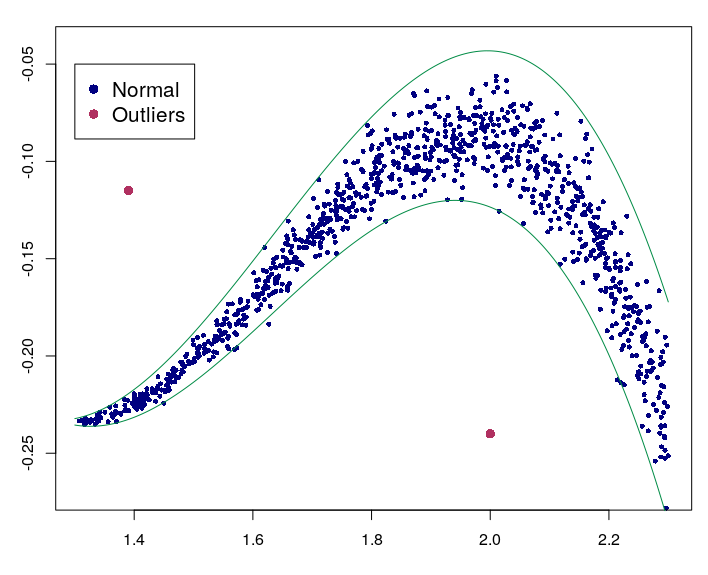
\includegraphics[width=\textwidth]{images/outlier_mine.png}
\caption{}
\end{subfigure}
\begin{subfigure}[b]{0.45\textwidth}
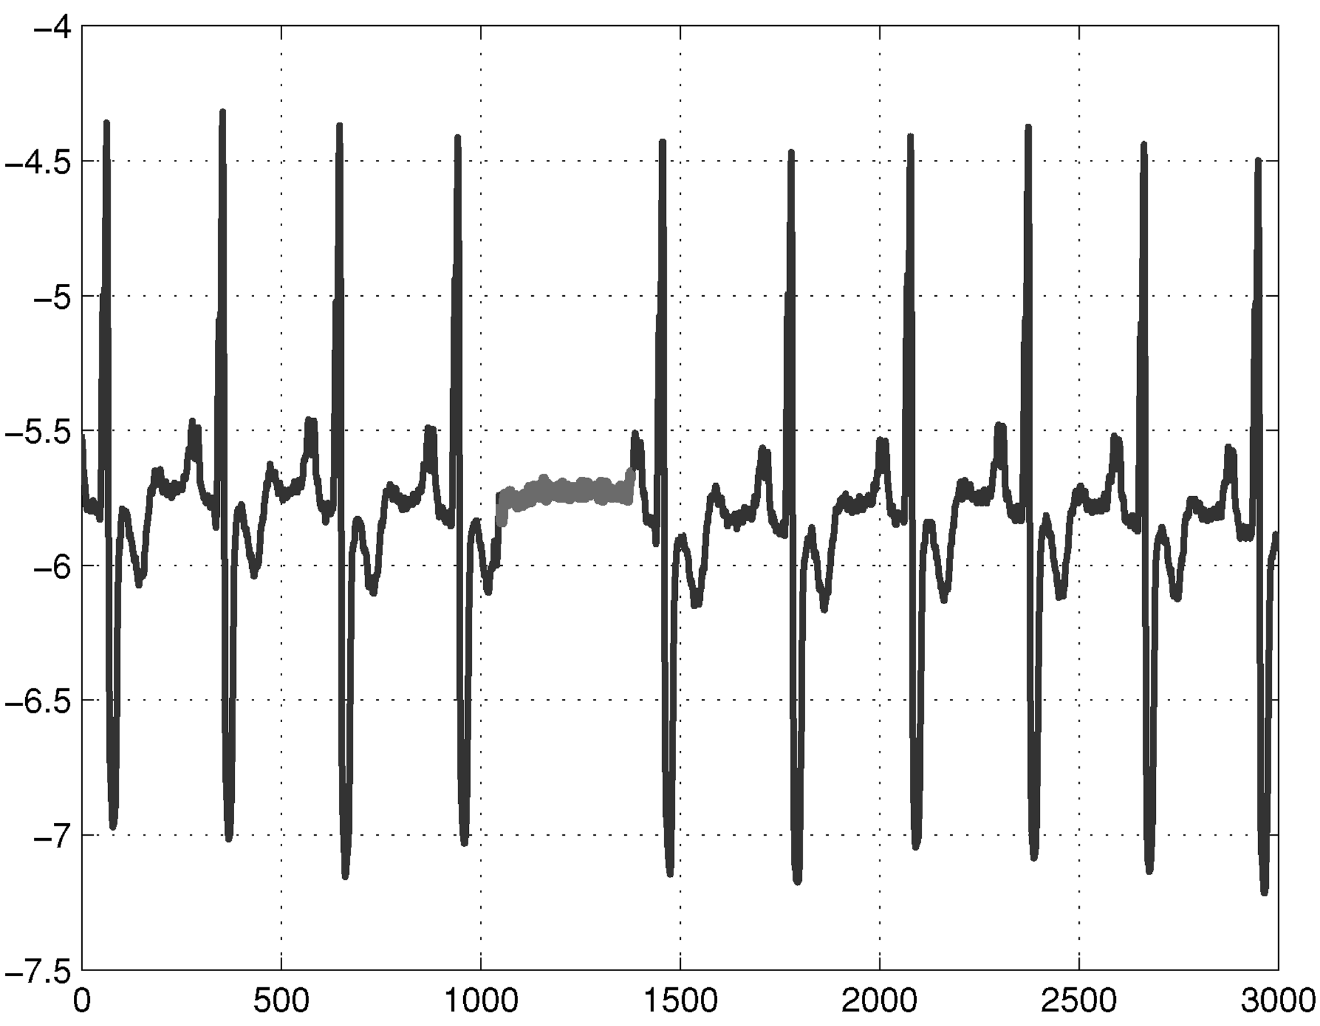
\includegraphics[width=\textwidth]{images/Atrial_Premature_Contraction.png}
\caption{}
\end{subfigure}
\caption{The left plot (a) depicts simple anomalies that deviate in distance from regular data. The right plot (b) shows a contextual anomaly where a group of data instances do not follow a repeating timely behaviour with respect to all other data points (corresponding to an \textit{Atrial Premature Contraction}, taken from \cite{chandola_anomaly_2009})}\label{graph}
\end{figure}

Anomaly detection has found wide application in areas where stability of  critical systems or detection of their abuse is crucial. Examples of these include engine-fault detection in wind-turbines, fraud detection for credit cards. The assumption here is that the modelled system, such as the sensor-data stream of an engine or the buying behaviour of a customer, remains stable and generates consistent data. Detected anomalies in new observations then indicate a potential fault or abuse in this system. Obviously, it is not inherently clear that every abuse or fault generates data that differs from normal data. Therefore, it is important to choose data sources that are able to reflect the unique nature of a particular system.

\subsubsection{Anomaly detection and NIDS}

Similar to the above described examples, anomaly detection has been applied to network security since the late 90's in order to assist IDSs. The behaviour of network computers are usually captured in the form of events logs such as network packets or flows, system calls, etc. The basic approach is to use collected training logs to infer a model of trustworthy activity, and then compare newly observed behaviour against this model. In order to prevent any anomaly model from learning malicious behaviour as normal, the used training data has to be free of any attacks. 
Again, the assumption is that unauthorized and malicious activity will correspond to behaviour that differs from trustworthy one. As an example, an anomally large network flow involving an unusual pair of network computers could indicate that a hacked computer is extracting or sending out sensitive data to an unauthorized destination. As an anomaly detection model does not make any assumptions about attack behaviour, but instead marks all deviations from the learned normal behaviour as potentially malicious, it is much better suited at finding novel and unseen attacks. However, features mined from the data have to be able to reflect normal behaviour in a way that malicious traffic will look different in order to detect it, which is not trivial. Furthermore, normal instances that only occur rarely or are diffuse will potentially also be flagged as potentially malicious, making an anomaly-based IDS prone to high false alert rates.



\section{Research opportunities}

As pointed out in my literature review, anomaly detection techniques currently perform best in the detection of attacks of larger volume, such as \textit{DoS attacks} or \textit{Port Scans}, and currently are the most common application in commercial IDS systems such as \textit{Hogzilla} or \textit{CFEngine}. In contrast, research on anomaly-based intrusion detection has been less convincing in the context of more targeted attacks that consist of only one or a few connections, with R2L (remote-to-local) and U2R (user-to-root) attacks currently being the least detected attack classes \cite{nisioti2018intrusion}. 

This can in part be explained by a lack of understanding of how these smaller, more point-like attacks differentiate themselves from normal traffic. Attacks using a larger number of connections will inevitably disturb the  distribution of one or multiple measures of the network, such as the byte-throughput or the port entropy \cite{lakhina2005mining}. However, an attacking connection inserting malicious code to gain control over a computer does not necessarily have different external properties\footnote{also caled \textit{connection summaries}} such as length, size, or port number, than the diverse range of normal connections. Yet, most attempts to detect these types of attacks via anomaly detection rely exclusively on summary properties of individual connections or packets to draw a border between normal and malicious traffic. Only very few approaches try to detect malicious connections as contextual anomalies, i.e. as traffic events that are not necessarily unusual on their own, but deviate from normal traffic in the context of their immediate temporal neighbourhood. Considering both the lack of literature in this area, this project will look more at the intrinsic nature of network traffic which is manifested in the \textit{semantic structure} of packet and connection sequences. 

Another pressing issue in anomaly-based intrusion detection is the problem of traffic evolution. An anomaly engine is usually trained once on a training set, and the learned notion of normal behaviour stays constant during the detection phase. There exist several approaches that can be trained in an online fashion, however none address the issue how new training instances are selected. This can lead to both high false alert rates when specific structures in the network change and to malicious traffic entering the updated training set. Sommer and Paxson identify this problem of non-adaptive models as one of the biggest problems in anomaly detection, naming it an area of tremendous research opportunities \cite{sommer_outside_2010}.


More information about about current state-of-the-art methods and identified literature gaps can be found in my literature review in Sections 3 and 4.2.

\chapter{Proposal}

\section{Project aim}

Chen et al. \cite{chen_2016_robust,chen_more_2016} recently demonstrated the effectiveness of state-based software models in the identification of malicious sequences actions in a stream of permission and API calls of Android applications. This usage of semantic features allowed the discovery of new malware instances and improved the overall robustness of the classifier drastically. 

This project will use the idea of semantic software models and apply it to network traffic data. It combines methods from machine learning and state-based software models, to automatically learn precise semantic models of network traffic generated by one or more machines. The semantic features of network traffic are here understood in terms of sequences of packet or connection metadata that correspond to fixed protocols of information exchange. These models together form a collection of normal semantic network behaviour of a network of machines, with malicious traffic being detected in an anomaly detection manner. Furthermore, a main aspect of this project will be to guarantee adaptivity and robustness of learned models to the evolution of software programs and their corresponding traffic. 

The motivation for the use of semantic models in network traffic stems from the fact that current anomaly detection methods perform poorly in the identification of temporally isolated malicious connections, as described above, as their external properties such as size, duration, or direction, do not necessarily deviate from normal traffic. Attacks containing such traffic often break into a machine by exploiting loopholes in the processing of program information, and thus in some way  break semantic structure of a communication. Traffic with malicious intent will therefore likely deviate in its intrinsic structure from benign traffic, and should be detectable when modelling this structure using semantic models.

Specific goals of this project are:
\begin{itemize}
\item Build an understanding of how semantic structures manifest themselves in network traffic.
\item Develop a semantic model of traffic structures that works on different levels of traffic abstraction (packets or flows) and enables the incorporation of semantic features from the packet level on a flow-level to extend available flow information.
\item Introduce adaptivity to anomaly-based models by identifying gradual changes in network communication as traffic with common semantic substructures.
\item Provide a framework to generate traffic data with a high level of ground truth about traffic origins and purposes.
\end{itemize}



\section{Work achieved so far}


\subsection{Data analysis and strategy}

Although this project is motivated by previous successful applications of ML-driven semantic models for anomaly detection, the differences in the type of data used in this project means that different tools and modelling strategies are necessary. Network traffic usually contains more intrinsic variation and noise, with packets potentially being dropped, and data distribution being afffected by the level of network congestion or by varying input parameters. Therefore, significant amount of time has been spent on initial data analysis and reflection on good modelling strategies. 

%Key assumption in this project is the following:

\begin{hypothesis}\label{Ass1}
Application $A$ running on a computer can be seen as a probability distribution $P_A(X)$ generating sequences $X$ of network events, with $X$ behaving as a random variable.
\end{hypothesis}

\begin{hypothesis}\label{Ass2}
Two applications $A$ and $B$ usually have different $P_A(X)$ and $P_B(X)$, which is applies especially to malicious applications. A computer running a set $N$ of applications %\footnote{including OS-applications}
generates sequences $X$ of network events with a distribution $P_N(X)=\sum_{n\in N}P_n(X)$. Consequently, a sophisticated and well enough trained anomaly model of a machine's traffic distribution $P_N(X)$ should be able to identify the existence of a new (and potentially malicious) application as traffic that did not originate from the set of existing applications $N$.
\end{hypothesis}

An additional assumption about systems we are looking at is that the set of installed software is relatively constant throughout the network, with new software installations being rather rare and controlled. 

\subsubsection{Semantic structures and corresponding variations}

Semantic behaviour of a program denotes how it transmits and reacts to information. This is can be observed both on a packet and on a flow level: Programs follow specific protocols on key-exchange etc. when a connection is established or how and with what frequency new bulks of data-packets are pushed, but also react to data retrieved in one connections with new connection requests such as the establishing of a HTTP-connection to an address received by an earlier DNS-request. Variation and noise are introduced in several ways:

\begin{itemize}

\item Varying sizes of data means a varying number and sizes of packets to be transmitted, which can in turn influence the way the receiver responds. Similarly, requested content can be made up of several files of different sizes which are transmitted in a varying number of connections with differing sizes.
\item Encryption can in a similar way introduce variation in packet or connection sizes and numbers.
\item Variation in the computational load or on the network on a computer can translate into varying response times to retreived information or much data is buffered and pushed at once. Similarly, packet loss or deviations from the established protocol by one side usually means that information has to be transmitted again.

\end{itemize}

A significant amount of time was spent at gathering appropriate  real-world data sources that can be used to train and to validate the developed methods. Due to its sensitivity, network traffic is not widely available. Furthermore, existing datasets are often subject sampling tools to reduce the amount of data collected, or are modified to preserve the privacy of the corresponding network users. Therefore, several datasets were analysed closely to establish whether they are suitable for both modelling semantic traffic structures and detection of malicious traffic. A summary of datasets can be found in the attached literature review in Section 2.2.


\subsection{Ground truth data generation}\label{Groundtruth}

Building semantic models of network traffic means to build an understanding how different network interactions can be distinguished via their traffic trace. We want to use ML techniques to automatically extract meaningful sets of sequences that represent these different interactions. In order to ensure that this is actually true, that our extracted models are indeed representing real distinguishable interactions and not just nonsense, we need validation from \textit{ground truth data}. 

Network traffic datasets are already hard to obtain due to privacy concerns. However, as  the correspondance between individual network traffic events and their particular purpose are virtually never recorded on a computer, their exist close to zero datasets containing ground truth about the contained events. For that reason, a particular aspect of this project is to generate useful ground truth data with appropriate content myself.

Over the course of the last year, Nikola Pavlov and I developed a framework that generates controlled and isolated network traffic from a variety of applications and tasks. For this, a virtual network was created using the virtualisation program \textit{Docker}. In this network, two or more parties can communicate as containers,  which are sandboxes containing programs inside a minimal virtualised operating system. The benefit of this design is that individual containers can only communicate with each other via the virtualised network while the host is in complete control of the parallel execution of tasks in multiple containers. In order to capture the traffic, every container in the network was complemented with a \textit{tcpdump}\footnote{A common packet capture utility}-container hooked onto the network interface. The captured traffic can then be labelled according to the particular scenario it was generated by.


\begin{figure}
\centering
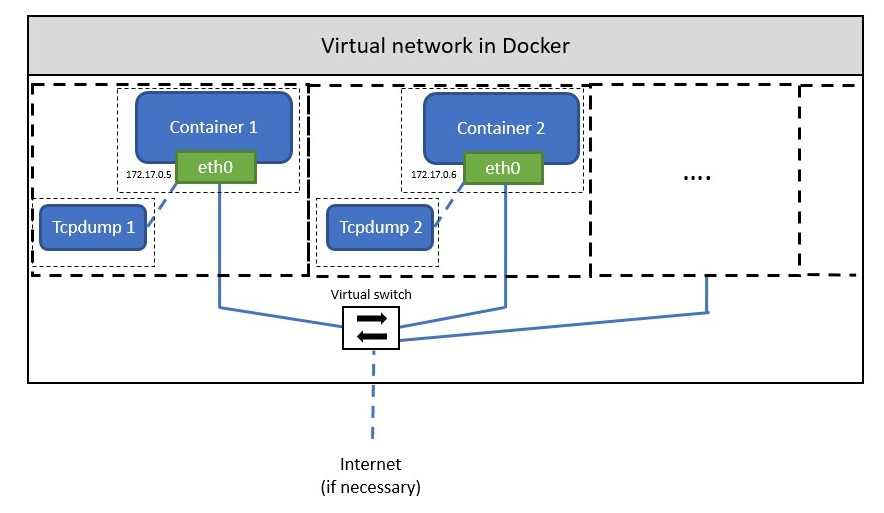
\includegraphics[width=0.7\textwidth]{images/Dockernet.jpg}
\caption{Visualisation of the virtual network in Docker}\label{docker}
\end{figure}

We implemented a variety of network service  scenarios to capture a diverse set of network traffic. Most, but not all, are set up in a server-client manner. Implemented services so far include:

\begin{itemize}
\item A simple \textit{icmp} ping service.
\item A \textit{nginx} server hosting a html-webpage with a client accessing it, both encrypted and unencrypted. Different client requests are implemented (\textit{wget} and \textit{Siege}).
\item An \textit{Apache} server hosting the same html-webpage with a client accessing it, also both encrypted and unencrypted. Again, different client requests are implemented (\textit{wget} and \textit{Siege}).
\item A \textit{Wordpress} server with a corresponding webpage and a client accessing it.
\item Different versions of an ftp server and client.
\item A mail transfer using \textit{mailx}.
\item An \textit{ssh}-server and client.
\item An \textit{IRC} chat server and two clients.
\item A file synchronisation service with multiple clients.
\item A web-crawler gathering a larger volume of traffic from the internet.
\end{itemize}

For each service, a number of different scenarios are implemented. For example, the \textit{ftp} client could pull, push, remove, or a combination of all one or multiple files\footnote{that might not exist}, or create a directory. Furthermore, randomisation is introduced on parameters like the file-sizes, request times, etc. in order to explore the dimensional variation of the traffic from individual actions.

To be scientifically consistent, the data generation should obey two basic principles: 
\begin{enumerate}
\item The execution of individual scenarios should provide consistent data. 

\item The data should be completely free from external influence, i.e. properties of or activities on the host machine should in no way disturb the data generation.
\end{enumerate}

Both properties were tested for selected scenarios with positive results. For the first, randomisation of the input was avoided as much as possible and the results of several scenario executions were compared. The second was tested by executing scenarios under differing workload and on different machines, and summaries over the different packet properties were tested using a Kolmogorov-Smirnov test. 


%\textcolor{red}{write about the application of the traffic, how to use it for validation}.


\subsection{Testing initial approaches on realistic data}\label{Prevwork}

In the context of the overall research goal of this project, some exploratory work on semantic anomaly detection for network events has been conducted by Marc Sabate, Gudmund Grov, Wei Chen, and David Aspinall. This work uses three different machine learning algorithms\footnote{A Markov Chain model, Finite-State Automata, and a Recurrent Neural Network} from the area of \textit{representation learning} to capture meaningful sequences of \textit{NetFlows} and reflect reoccurring patterns in a model. For that, recorded NetFlows are grouped according to the generating host. Furthermore, in order to filter out sequences of flows that are unrelated to each other, a squence of flows that are close in time is grouped into what is called a \say{session} as an approximation \say{true relation}. Each session then serves as a training or test sequence for a behavioural model. Learned semantic behaviour is reflected through the capability of the model to predict traffic protocols and network ports of flows in a session from a smaller subset of flows, with more accurate predictions being rewarded in the training process. Sessions which deviate from previously observed behaviour are then predicted poorly by the model and flagged as potentially malicious.

\begin{figure}
\centering
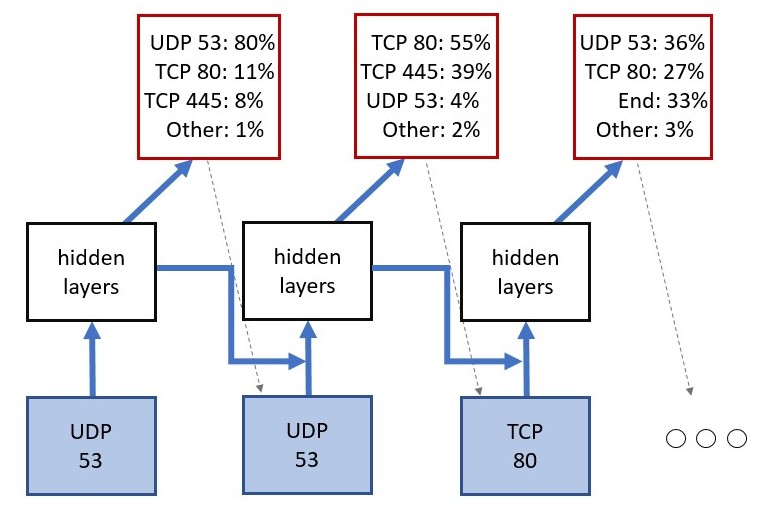
\includegraphics[width=0.7\textwidth]{images/RNN.jpg}
\caption{Visualisation of the RNN-method used}\label{RNN}
\end{figure}

%\textcolor{red}{maybe write about how these methods are directly relevant for this PhD and could be extended, improved or incorporated}.

The described methods were tested on the CTU-13 dataset \cite{garcia2014empirical}, a laboratory generated dataset available to study botnet detection. The great benefit of this data is the inclusion of both benign background traffic, on which the models were trained, and malicious traffic used to test their detection capabilities, and the availability of corresponding labels. Furthermore, it consists of more than ten million flows on multiple machines, thus containing reasonably much variation for testing purposes.

Anomaly-based methods in intrusion detection are often criticised for working only in controlled environments while failing in the real world. To counter this criticism, it is crucial to provide evidence of success on sufficient data gathered under realistic conditions. For the CTU-13 dataset, the generation of both types of traffic was done in a controlled laboratory environment, making it a so called \say{synthetic} dataset. This does not necessarily mean that it does not reflect realistic behaviour, however there is no guarantee that it contains all variations encountered in an operational environment. 

In order to bolster the findings of this sub-project, I applied the same methods on currently available real-world datasets which I am already familiar with through my MSc thesis \cite{clausen2018bayesian}. The particular datasets come from the enterprise network of the \textit{Los Alamos National Laboratory} \cite{kent-2015-cyberdata1} and from a Spanish ISP \cite{macia2018ugr}. For that I selected appropriate machines (e.g. IP addresses) that contain the variety of traffic behaviour found on personal computers, in contrast to less diverse traffic sources such as IP-phones, printers or servers. Furthermore, the selected machines should be subject to attacks so that the effectiveness of the results can be verified. I made sure the data is in the right format to be passed to the implemented models and supervised the training process by adjusting important parameters and hyper-parameters. Finally, I evaluated the results and added them to the existing manuscript.

\section{Research questions}\label{RQ}

Chapter 2.1 described the broader motivation and ambition for this project. To achieve a coherent scientific progress, this PhD-project will explore the problem of modelling the semantic behaviour a computer from different angles and hopefully find answers to the most important questions that arise in the process. Below I formulated four questions with a number of sub-questions that address different parts of this project and will be central for my work.

\subsubsection{Data analysis and exploration}

Network traffic is a form of communication between computers, but in our case it is also an observed signal of unobserved computational actions on those computers. This signal does not contain all semantic information of those actions and could potentially make them indistinguishable. 
However, we assume that a reasonable amount of distinct semantic structures will be translated to the corresponding traffic generated by an action.

As the space of and structure of the modelled data is of immense importance for anomaly detection, I wis to answer the following questions:

\begin{rquestion}
How well-structured is the space of semantic behaviours observed in the traffic  machine or a network structured? 
\begin{enumerate}
\item How can we scientifically quantify closeness between individual actions, and does it translate into the similarity of corresponding traffic structures? 
\item How much does noise or input variation blur the observable semantic differences between distinct actions?
\end{enumerate}
\end{rquestion}

\subsubsection{Modelling scope}

Anomaly-based detection systems aim to find deviations from normal behaviour in as many ways as possible. For that, it is desired that any semantic model of network traffic should represent common network traffic with as much information as possible. However, a too detailed model runs the risk of being of overfitting the structure found in the training data and consequently yielding high false-alert rates. Therefore, we need to address the following questions: 

\begin{rquestion}
To what degree can semantic structure in network traffic be captured in a model from a training dataset, and how can we achieve this?
\begin{enumerate}
\item Which parts of network traffic both contain important information and can be represented by a model?
\item Can be combine models that act at different traffic levels to enhance the amount of context given by the data? 
\item Can we efficiently disentangle overlaying network flows to isolate otherwise distorted flow groups corresponding to similar actions? 
\item What is an efficient and realistic way to incorporate other data sources into the modelling procedure? How can this input enhance the learning process and the representation detail of a traffic model? 
\item How can a model adapt to changes of normal semantic structures?
\end{enumerate}
\end{rquestion}

In order to capture the diversity of network traffic, large quantities of training data will need to be processed. The choice of modelling methods will therefore depend on several aspects such as computational efficiency, retraining capabilities, and interpretability.

\subsubsection{Ground truth data and evaluation of semantic understanding}

Identified semantic structures in network traffic should represent semantic behaviour of programs on a computer to be meaningful and applicable for the detection of malicious network behaviour. A ground truth about the program or service that generated particular network events is partically non-existent in available datasets. In order to evaluate the representation of traffic structures a given model provides in a more comprehensive way than via the detection rate of known malware instances in a dataset, I want to answer the following question:

\begin{rquestion}
What is a meaningful representation of traffic structures?
\begin{enumerate}
\item What requirements must a labelled traffic generation framework fulfill to provide realistic data?
\item Can we evaluate the traffic representation of a model through its ability to identify semantic closeness between traffic instances correctly?
\item How can we quantify the capability of a given traffic model to identify new computational actions on a machine?
\end{enumerate}
\end{rquestion}

\subsubsection{Application to realistic Intrusion Detection}

Finally, this work should make an impact on future intrusion detection methods. Although anomaly-based methods are meant to be agnostic of a notion of malicious activity, we have to ask how and where this work will offer improvements in the detection of modern attacks. In order to effectively increase detection rates, semantic anomalies have to occur within attacks that are not reliably detected yet and are not trivial for an adversary to disguise our hide. 

\begin{rquestion}
What will a semantic model be able to prevent? 
\begin{enumerate}
\item What kind of attacks will necessarily show semantic anomalies, and which will not?
\item Can an adversary adapt his attacks to avoid detection? How can we prevent this?
\end{enumerate}
\end{rquestion}

\vspace{0.8cm}

These questions will drive the direction of my research during this project. I do not expect to address all of them comprehensively, but I believe that I will be able to find satisfying answers to the majority. In the next chapter, I am proposing specific sub-projects that will pave the way to find scientific results for questions in each of the different areas.


\chapter{Project specific objectives}\label{Obj}

\section{Learning representations of packet exchanges}\label{Repr}

%\textcolor{red}{As became clear during our investigation}
The distinct semantic behaviour of an applications manifests itself most clearly in the first few packets exchanged in a connection. This is the stage in a connection during which a specific client or server request is transmitted, encryption keys are exchanged, users authenticate themselves with passwords, ports for successive connections are defined, etc. This distinction goes far beyond individual traffic protocols, as even a single application usually can exert different actions which translate to different semantic behaviours in this initial negotiation phase. 

The significance of the initial negitiation phase is bolstered by two publications on the area of traffic classification that share the same conclusion and train clusters and classifiers on the metadata of the first five to ten packets to distinguish different applications \cite{bernaille2006traffic,crotti2007traffic}.


\begin{figure}\label{negot}
\centering
\begin{subfigure}[b]{0.49\textwidth}\label{FTP}
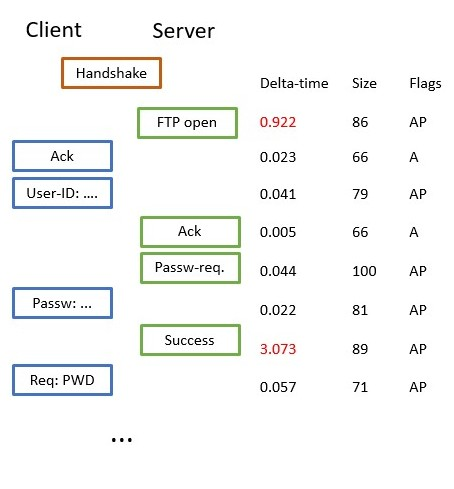
\includegraphics[width=\textwidth]{images/FTP.jpg}
\caption{}
\end{subfigure}
\begin{subfigure}[b]{0.49\textwidth}\label{SSH}
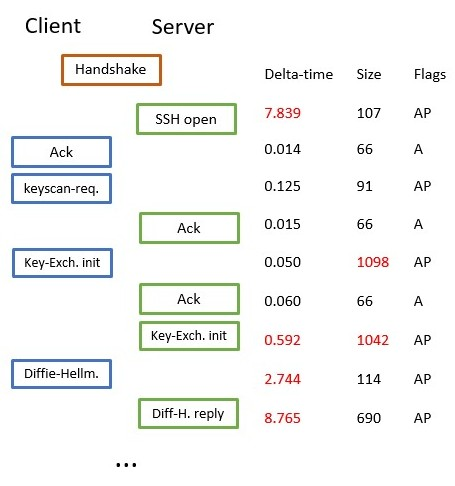
\includegraphics[width=\textwidth]{images/SSH.jpg}
\caption{}
\end{subfigure}
%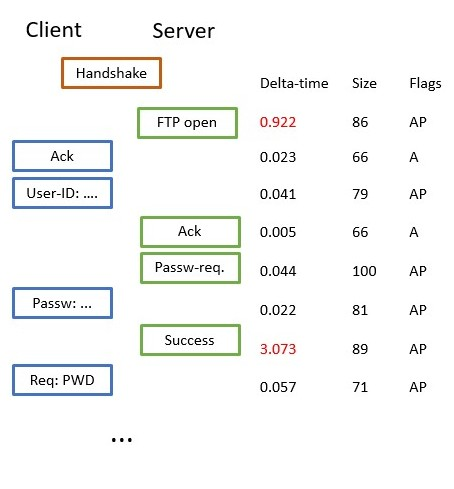
\includegraphics[width=0.7\textwidth]{images/FTP.jpg}
\caption{Depiction of user-ID and password exchange in an FTP-connection (a) and an SSH-connection (b) during the negotiation phase.}
\end{figure}

%\textcolor{red}{write about why this work needs to be extended with more sophisticated models (there is some text in Bernaille about flaws)}



Learning precise semantic representations of this initial negotiation phase from applications running on a computer has several main benefits for this project: 

\begin{itemize}
\item Several types of attacks exploit loopholes accessible at the negotiation stage. A precise semantic representation model could detect anomalous deviations in particular packet parameters from the learned behaviour. A simple example of such a deviation from expected behaviour would occur during a \textit{buffer overflow attack}, which overflows an input buffer (such as for a password) to directly modify memory locations. This should be observable as a significant deviation in the corresponding packet size.

\item Newly installed malware will most likely exhibit different than normal behaviour in this stage, from very different negotiation procedures to just slight deviations in the packet interarrivals.

\item The translation of semantic negotiation structures into different behaviour groups could be used to associate the corresponding flow with particular actions, i.e. to give the flow one or more labels. To be meaningful, the identified groups have to correspond to actual semantic behaviours and should be consistent along similar actions. 
Such a flow labelling could be very helpful for understanding semantic structures of flow traffic, and consequently for anomaly detection on a higher level, such as the described work by Chen et al.\cite{chen_more_2016}. I will describe this more in Section \ref{Curmet}.

\item As applications are updated, their particular traffic generation distribution $P(X)$ can also  gradually change, causing corresponding traffic to be potentially flagged as anomalous by current anomaly detection methods. A representational model could identify common semantic substructures between traffic instances and thus indicate that they originate from an updated application. More detail will be given in Section \ref{Robustness}.

\end{itemize}

Focusing exclusively on this initial phase, i.e. a fixed number of the first packets in a connection, has several benefits: We are dealing with a fixed and comparibly small input size, which lower computational cost and is beneficial for modelling techniques with a higher complexity. Our model is tainted by large data exchanges, which usually do not contain as much useful information but are spread across many more packets, which could create a high imbalance in the traffic representation. And we do not have to wait until a connection is finished for its evaluation.

A model that offers enough representation of semantic structure has to go further than the above mentioned work, which was intended for traffic classification instead of cyber-security. Therefore, I propose two unsupervised modelling approaches that are intended to encapsulate significantly more information.

\subsection{Probabilistic Real-Time Automata}\label{PRTA}

The \textit{non-deterministic finite-state automaton (NFA)} is a widely used model for discrete event systems and can be seen as a mathematical model of computation. It is a type of Markov chain with a finite number of states and a set of Markovian transition probabilities from each state to the others. A recent variant of the  of the NFA is the \textit{probabilistic real-time automaton (PRTA)}, which models the event interarrival times as a discrete distribution that is dependent on the current state. 

Automata are learned from a set of input sequences via state-merging. In this procedure, a trie with all observed event sequences is built, with each path in the trie representing one input sequence. Pairs of paths that are close to each other are then merged, thus generalising over the input data and learning the structure of the target machine. Closeness is determined by heuristic measures, with a merge  considered good if the future behaviour after  reaching state $p$ in one path is  similar to that after reaching $q$. Figure \ref{Autt} depicts this process.


\begin{figure}
\centering
\begin{tabular}{c}
\begin{subfigure}[b]{0.85\textwidth}\label{Autotrie}
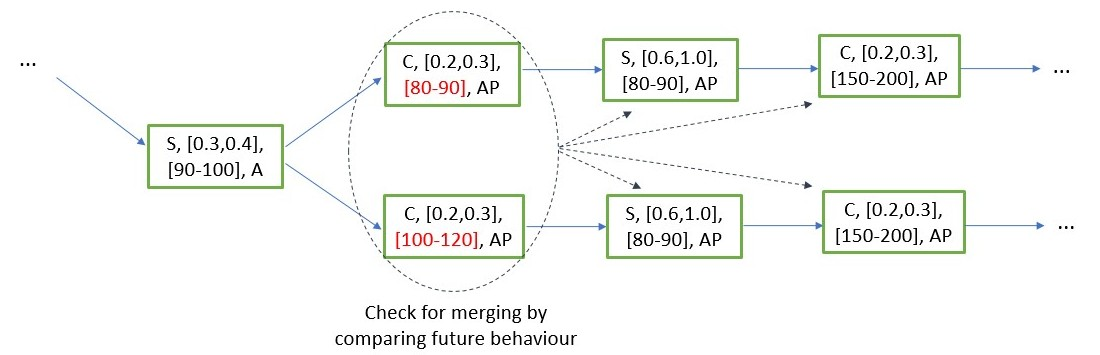
\includegraphics[width=\textwidth]{images/Autotrie.jpg}
\caption{}
\end{subfigure}\\
\begin{subfigure}[b]{0.85\textwidth}\label{Automerge}
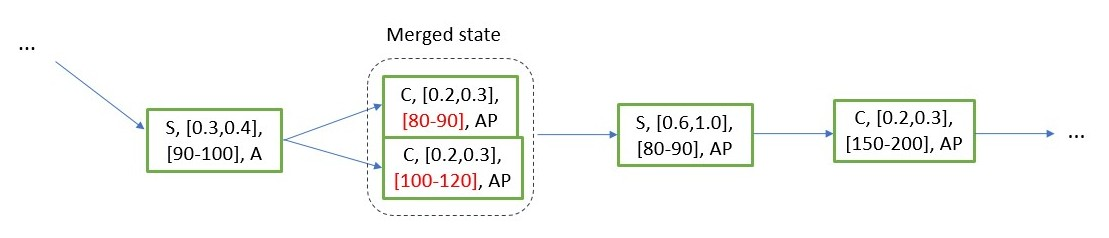
\includegraphics[width=\textwidth]{images/Automerge.jpg}
\caption{}
\end{subfigure}
\end{tabular}
\caption{Depiction of the state-merging process for two input sequences}\label{Autt}
\end{figure}

As the exchange of network packets is a symbolic sequences of a computational process, they are a very suitable candidate to be modelled by probabilistic automata: The tree-branching in an automata is well suited to represent the different avenues a negotiation can take while the probabilistic state-merging ensures that potential variation within one avenue are accounted for. With enough traning data, automata can therefore provide a much more refined representation of a given set of packet sequences than previously explored techniques without overfitting. Anomaly detection to identify potentially malicious traffic can then be done by computing the likelihood of a input sequence trajectory and flagging it if it false a likelihood-ratio test. 

Using probabilistic automata has further benefits in the context of this project. In contrast to many methods, they are interpretable by domain experts when checking, which is a priority for many researchers in order to process the inevitably\footnote{due to the inbalance between benign but irregular traffic compared to actual attacks} high occurrencies of false alerts. Furthermore, the branching structure in automata provides a natural grouping of sequences, which can be used to engineer labels for similar sequences in a similar manner to the \textit{hierarchichal clustering method}. Such labels can be very useful in future ambitions discussed in Section \ref{Curmet}.

PRTAs have been applied to network traffic before by Pellegrino et al. \cite{pellegrino2017learning}, however in a different context and scale. To apply automata to this project, network packets would have to be transformed to discrete, finite states. Interesting properties to be included are 

\begin{enumerate}
\item the direction of the packet,
\item TCP-flags,
\item the interarrival time,
\item the size of the payload,
\item and potentially the offered window size.
\end{enumerate}

To create states, continouos variables have to be transformed into a set of finite non-overlapping intervals. For a better resolution, a rescaling onto a logarithmic scale is very sensible. The combination of all attributes into one set of states is then straightforward. 

One challenge in this project is the large amount of training data needed to represent the variability of network traffic. Schmidt and Kramer \cite{schmidt2014online} have recently proposed an online learning approach for PRTAs that enables the effective processing of massive datasets, which could be very useful for this project. A further thing to consider is that the chosen similarity measure for state-merging should be able to account for additional \textit{ack}-packets inserted in the connection or potential packet loss. A possible solution is to introduce non-vanishing probabilities for both scenarios, i.e. it should be possible from every state to jump to an empty \textit{ack}-packet and back, or to skip a packet. Another solution which could also reduce the potential computational burden is to learn multiple automatas from the input using rolling windows over, with each automata learning a specific interval of the negotiation phase, in a similar manner as in \cite{pellegrino2017learning}. This could increase the stability of individual automata and decrease the size of the trie. Furthermore, as each automata would correspond to sub-behaviours in the connection, it would be possible to identify common subsequences in traffic from updated software and thus create a relation to previous traffic. 

\subsection{Autoencoder-based}\label{AUTOBASED}

\textit{Autoencoders} are the most popular deep learning-based method for unsupervised representation learning. They can learn a compressed representation of input data by self-supervised training using the reconstruction error of the input data. Although autoencoders themselves do not produce a defined model of the input data, they translate complex structures into a more simple space in which they can be described by conventional density estimation methods. 

\textit{Long short-term memory (LSTM)} autoencoders are a recent version of autoencoders that use the structure of RNNs to capture the sequential nature of the input data before the encoding-process, first introduced by Srivastava et al. \cite{srivastava2015unsupervised}. Since then, they have been successfully used for artificial creation of facial videos, music generation, or for text compression.
LSTM autoencoders can be trained using backpropagation, and the application of an LSTM autoencoder to packet data is straightforward, however again time and size variables should be logarithmically rescaled. Anomaly detection can then either be performed by thresholding the reconstruction error of new input sequences \cite{malhotra2016lstm}.
 
\begin{figure}\label{LSTM_Enc}
\centering
\begin{subfigure}[b]{0.65\textwidth}\label{LSTM1}
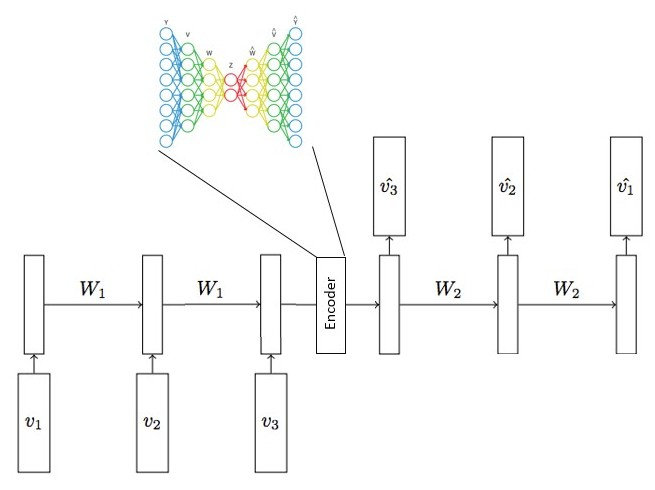
\includegraphics[width=\textwidth]{images/LSTM_Encoder.jpg}
\caption{}
\end{subfigure}
\begin{subfigure}[b]{0.34\textwidth}
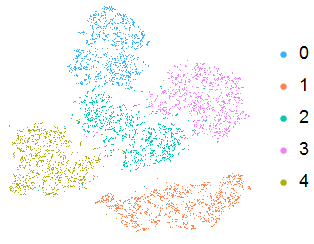
\includegraphics[width=\textwidth]{images/MNIST.png}
\caption{}\label{LSTM2}
\end{subfigure}
\caption{Visualisation of the design of an LSTM Autoencoder (a), taken from https://machinelearningmastery.com/lstm-autoencoders/, and the embedding of different types of handwritten digits by an autoencoder.}
\end{figure}


LSTM autoencoders are an excellent alternative to PRTAs for the modelling of packet data due to their superb ability to discover non-linearities in sequential data, and the fact that they can be trained on massive datasets. They have been used to discover semantic structures before both for natural languages \cite{yang2017improved, silberer2014learning} and computational sequences \cite{yousefi2017autoencoder}.
 Furthermore, the embedding of input data into a lower dimensional continuous space means that clustering of similar traffic instances to create higher level flow labels can be performed, see Figure \ref{LSTM2}.

\subsection{Data and result validation}\label{Resultsval}

The above described methods should be tested for three properties:

\begin{enumerate}
\item Goodness of fit,
\item detection capabilities of malicious behaviour,
\item correspondance of engineered high-level labels to actual semantic behaviour.
\end{enumerate}

Testing of the first two properties is straight-forward given a suitable dataset. Goodness of fit could be tested with any packet data collected from a suitable environment and could even be generated for the experiment. To test detection capabilities, a packet dataset containing labelled malware traffic  is necessary. Two widely used datasets, the CICIDS 2017 and the UNSW-NB 2015 dataset are suitable candidates \cite{moustafa_unsw-nb15:_2015,sharafaldin2018towards}.

The third property is not as straight-forward to test, as hard ground truth about the purpose of individual connections is required to analyse the labelling consistency. Fortunately, such ground truth data is now available to us for a variety of services by our data generation tool, described in Section \ref{Groundtruth}. To test the labelling consistency appropriately, a given dataset could be superimposed with labelled ground truth traffic, and split into training and test data. If individual scenarios in the test set are both identified consistently  while associated with a different label than significantly different scenarios, the labelling can be seen as meaningful.  


\section{Software evolution and drift}\label{Robustness}

Networks and their corresponding traffic are not static, but gradually change over time. Consequently, making intrusion detection systems adaptive to such changes in normal behaviour is an increasingly important issue in the research community \cite{sommer_outside_2010,noble_real-time_2018}.

In our context, such changes in normal behaviour would appear in the observed semantic structures and could be induced by new software being installed on the observed machine, or by installed software changing through updates or similar modifications. As new software could equally be of malicious nature, there is no way to make our system robust against such changes without introducing additional notions of overall malicious software.\footnote{which is why we are assuming that new software is not installed on a regular basis} 

Software updates however should correspond to more gradual changes as only small parts of the software are modified. Hence, it is reasonable to assume that in the process only parts of the semantic traffic structure will change, while larger parts surrounding it stay the same. %\textcolor{red}{give an explaining example of this}
A logical approach to distinguish this gradual software evolution from more abrupt changes would therefore rely on the comparison of semantic sub-features to detect an overall closeness between traffic instances. However, more analysis of traffic evolution under software updates has to be conducted to make reliable statements about precise modelling methods. Yet, a few ideas are presented here.

Chen et al. \cite{chen_more_2016, chen_2016_robust} introduced the concept of common sub-automata between similar malware instances in order to improve the robustness of detection methods. This notion could be used in this project in a similar way: Traffic instances deviating from the learned traffic automata are examined for sub-automata that are within the learned range of normal behaviour, depicted in Figure \ref{Robust}. If enough common sub-automata exist, the traffic is marked a potential software update and either authorised by an administrator or directly incorporated into the existing model. 

\begin{figure}
\centering
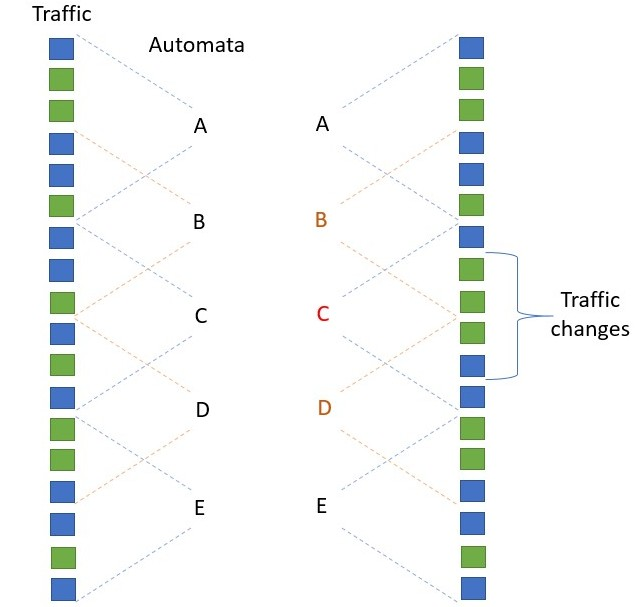
\includegraphics[width=0.5\textwidth]{images/Robust.jpg}
\caption{Depiction the comparison of sub-structures between two traffic instances.}\label{Robust}
\end{figure}

Depending on the exact implementation of methods proposed in Section \ref{PRTA} and \ref{AUTOBASED}, there are several ways to design such a comparison. In case a rolling window based approach to learn traffic automata is chosen, a comparison between automata from different time-intervals is straightforward, with  heuristic measure to decide on an overall closeness to be chosen. If instead complete traffic automata are learned, Chen et al. proposition for a machine-learning-centred algorithm to efficiently choose salient sub-automata could be used. For an autoencoder-based approach, successive traffic sub-intervals can be mapped into lower-dimensions, with their distance to the normal region indicating if each interval corresponds to normal behaviour or not. 

\subsection{Evaluation}

In order to gather data and to test developed methods, I will again make use of our ground-truth traffic generation framework. For that, containers with different versions of the same software will be installed and the corresponding traffic will be gathered. Next to initial data analysis, this traffic can then be injected into real-world datasets in a similar fashion as described in Section \ref{Resultsval}, with traffic from older versions being injected into the training data while that from newer versions into the test data. Such a dataset can then be used as a benchmark to test the ability of the above described methods to identify traffic from newer software version as such. 

The data produced this way does not necessarily represent the influence of software updates on network traffic as a whole. However, it can give good indications of the amount of change introduced and is a good testing possibility for our methods in a very novel area of cyber-security until more extensive datasets become available. 

\subsection{Adaptive learning}
Despite the identification of similar traffic instances, their incorporation into the existing model without introducing concept drifts or catastrophic interference is an important task. Online or incremental learning methods exist for both autoencoders and PRTA and could be used with new traffic gathered over time. However, special attention has to be paid to the fact that once traffic from updated software is identified, it should be included into the model immediately to avoid a flood of traffic alerts from the same software. How this this specific problem can be solved will depend on specific models and is yet to be determined.

\section{Flow-level based modelling}\label{Curmet}



In Section \ref{Prevwork}, initial work by Aspinall et al. on modelling semantic traffic structures on a flow level is described. This work demonstrates that semantic structures in a machine's network traffic can be observed on a flow level, and how these can be used to identify malicious behaviour as deviations from normal behaviour.

As this work is an initial step towards a flow-based semantic models, there is room for further developments and improvements which are congruent  with the general aim of this PhD-project, in particular with . I therefore propose the following measures to create a more detailed and precise traffic model:


%With the exception of the work by Aspinall et al. described in Section \ref{Prevwork}, only little literature exists about the semantic structures observed on a network flow level. Asppinall et all exception


\subsection{Combination of packet and flow-level information}

The current traffic models by Aspinall et al. only incorporate protocol and port numbers of successive flows as semantic features. Network flows additionally include the IP addresses of contacted machines, the direction of the connection, and strongly correlated information about the duration, size, and packet number of a flow. Network flows additionally include the IP addresses of contacted machines, the direction of the connection, and strongly correlated information about the duration, size, and packet number of a flow. Both the direction and the duration or size of a flow are readily available quantities that could help identify more detailed substructures. However, all these parameters describe a flow on a quite high level of abstraction, with a lot more information about the type of traffic not being captured. This information gap is widely recognised in traffic classification research, with a number of approaches generating additional connection information such as interarrival or packet size statistics. Including such information would be a fairly straightforward choice to improve existing methods. I however am more interested in examining how semantic information about a connection could be used to give sequences on a flow level more context.

This task is in direct correspondance to the posed research question 2.2: \say{How can we combine models at different traffic levels to enhance the amount of context given by the data?} This question is very important in regards to extending a systems capability to detect anomalies effectively. Events in a network can be disturbed by many factors, and the space of events accepted has to included many rare, albeit possible events as normal. This could for example mean that a TCP hijacking attack is for a model indistinguishable from a connection malfunction. However, such an event at packet level will likely trigger some effect on the flow level, like the opening of a similar follow-up connection etc, which might not necessarily be the same if the event was malicious. If the context of a malfunction or similar event inside a connection would be available to models on the flow level, their expected effect could be compared to the observed one to receive a greater level of detection capabilities.


How this combination of semantic packet and flow level information would be implemented will depend on the outcome of the project described in Section \ref{Repr}. A fully connected model that learns information structures at both levels simultaneously would be desired as learning and updating would be more natural and cause less problems in the information linking. This is however not the only possible way to proceed as a stacked combination of two models where training is performed independently could be an easier solution to implement and test.

In Section \ref{Repr}, I described how a model of packet exchanges can be used to automatically create connection labels for different groups of semantic behaviour, both using PRTA and autoencoders. These labels would describe a greater subdivision of traffic types in similar way to common network ports which already give a broad indication about the type of traffic. As the currently used methods already work with port numbers, it would be straightforward to extend them on these artificial flow labels.


\begin{figure}\label{LSTM_Enc}
\centering
\begin{subfigure}[b]{0.45\textwidth}
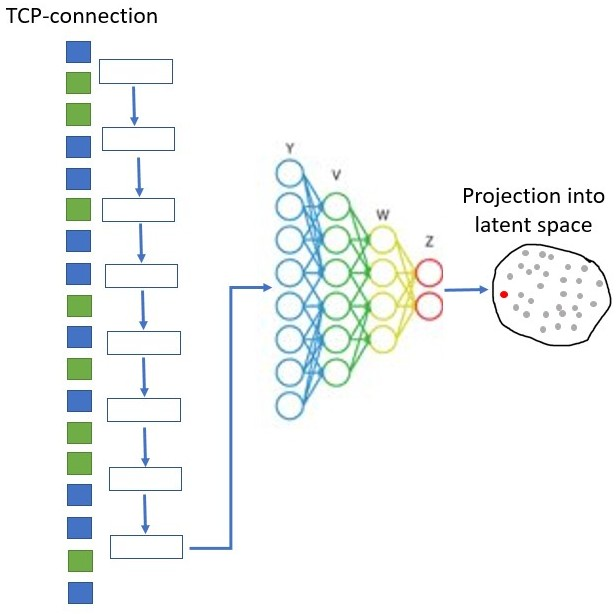
\includegraphics[width=\textwidth]{images/Latspace1.jpg}
\caption{}\label{Lat1}
\end{subfigure}
\hspace{0.5cm}
\begin{subfigure}[b]{0.45\textwidth}
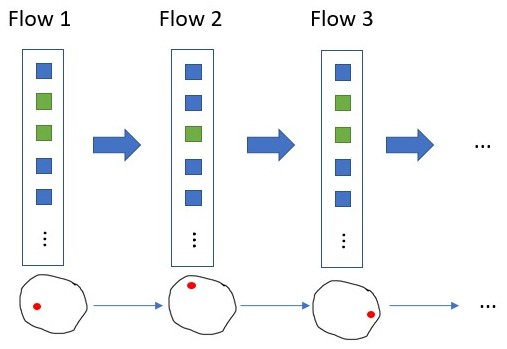
\includegraphics[width=\textwidth]{images/Latspace2.jpg}
\caption{}\label{Lat1}
\end{subfigure}
\caption{Visualisation of the use of extracted semantic information from the packet level (a) to be used in modelling sequences of flows (b).}
\end{figure}

\subsection{Traffic separation}\label{Sep}



The described current models are representing semantic structures as the prediction accuracy of the next element in a sequence, as depicted in Figure \ref{RNN}. This probabilistic method is quite effective when semantic sequences are isolated, even under noise, as can be observed in current language models \cite{shi2012towards}. This is however not always the case in a stream of network flows as two or more independent actions generating traffic can have temporal overlap, causing their corresponding semantic structures to overlay each other. Subsequent separation of the different signals is a hard problem and at this stage likely infeasible. Since these overlays can occur between completely independent actions, it is hard for our current models to accurately predict the next event in an overlayed session. Although these traffic overlays appear to not be the norm in a machine's network stream, the decrease in prediction certainty in a session depletes the possibility to detect anomalous behaviour and thus opens a door a door for adversaries to hide attacks in normal traffic. 


The problem of separating traffic from different services itself is computationally not trivial, and there may not exist complete solution. It is still however still worth to consider possible ways to isolate significant traffic instances, or how to at least improve robustness of existing solutions. The traffic generation framework described in Section \ref{Groundtruth} can be very beneficial for this taks as we can generated overlayed traffic with the ground truth labels of the different traffic signals. 

\subsubsection{Training a classifier}

One possible idea I would like to explore is to generate a larger quantity of overlayed traffic sessions with corresponding signal labels and a realistic level of variation to train a classifier. This classifier should try to put flow events into groups according to their generation source based on group properties observed in their IP-addresses, sizes, etc. As labels will be provided, this task can be done in a supervised manner. The learned distinction distinction properties should be general enough to be applied to different traffic tasks. 

In order to support the learning process, data from other sources such as application logs or operating system calls could and should be used. More information on how these could be generated can be found in Section \ref{Fusion}. 

If the classification of network events into groups is too hard, the classifier could instead be trained to just identify if a session contains overlayed traffic or is generated by one source, which could inform a detection system of the ambiguity of the observed session. 

How exactly an appropriate classifier could be designed is still to be determined. 



\subsubsection{Robustification}

If the separation of signals turns out to be too difficult, it is still possible to improve the existing RNN model and increase prediction accuracy of overlayed events in a session:

\begin{itemize}
\item Instead of predicting one successive event in a sequence, prediction accuracies of an RNN can be improved by extending the prediction to multiple unordered events that are supposed to occur within a window. This will shift the focus from one event which is relatively unpredictible under overlay to a larger group in which particular events are relatively certain to occur. This way, a model can learn semantics easier and can provide a higher certainty under overlays.
\item  For longer sessions, a rolling window approach should be introduced. This way, hidden neurons can be reset easier and adjust to the current behaviours in a session. This is helpful when one behaviour is directly followed by a different independent one.
\end{itemize}





\section{Traffic generation and data fusion}

To build meaningful semantic models, it is essential to compare discovered traffic features with the corresponding actions the traffic represents, for which ground truth traffic is necessary. Our data generation framework described in Section \ref{Groundtruth} is to our knowledge the first of its kind in the way that every generated packet or connection can be linked to a specific application and the specific task that application completed. This framework might not only be beneficial fo us, but also for other researchers interested in data with a high level of explanatory labelling.

In order to harness the unique opportunities this framework is offering on ground truth data generation, I hope to extend it in the following ways:

\subsubsection{Simulate real network traffic distributions}

As many network intrusion detection methods are designed for application to enterprise network traffic from personal computers, it is reasonable to evaluate them on traffic that has similar characteristics. As network traffic\footnote{at least on an IP level} consists of traffic originating from a set of applications performing different tasks, we can try to simulate network traffic on a machine by generating sequentially traffic instances from each scenario from a probability distribution specific to that scenario, and  pooling it into one traffic stream. For that, the following questions are interesting to us:
\begin{enumerate}
\item What kind of applications and services are typically responsible for the generation of typical enterprise network traffic on individual machines?
\item Into which generalised subtasks can these services be broken down?
\item How can we quantify the frequency of each application generating traffic?
\item What other underlying traffic properties such as service correlations or network congestion did we not capture?
\end{enumerate}

\subsubsection{Data fusion}\label{Fusion}

Apart from network traffic, applications often produce additional events captured in log files. These are usually intended to control whether a service is working properly, but are also increasingly used for cyber-security purposes. The fusion of multiple events streams such as log files and network traffic is a very promising direction in current intrusion detection as the combination of multiple indicators for malicious activity has the potential to significantly decrease the rate false positives, and some effort has been made to provide synchronised data sources, notably from the Los Alamos National Laboratory \cite{kent-2015-cyberdata1}. However, it is traditionally very hard to link specific log events with corresponding network traffic events due to the lack of ground truth traffic. Due to the separation of traffic from individual applications and programmable execution of different scenarios, our framework can provide the unique opportunity to examine and model this relationship. %In this PhD-project I hope to contribute in the following way: 

%\begin{enumerate}
%\item Implement a synchronised and time-stamped generation of traffic and log events for particularly interesting scenarios.
%\item Develop a parsing tool that can 
%\end{enumerate}
%\subsection{Interpretability}

\chapter{Programme of work and potential risks}

Section \ref{Obj} presented a number of different subtasks this PhD-project will be split into. I will now give an outline of my workplan of this series of interdependent workpackages, which will be carried out in parallel. The outlined plan of work is relatively conservative to accomodate enough time for different tasks. I expect that several projects will be completed sooner and that additional room for further work on the reserach question in Section \ref{RQ} will be conducted.

\subsubsection{First year}

The first half of year one was spent on reviewing literature, data collection, and evaluation of research opportunities. The results were used to produce both a comprehensive literature review and this document. Besides this, I attended a one-week data study group at the Alan Turing institute in the context of knowledge exchange and skill development. While there, I contributed in the creation of a comprehensive report on \textit{Developing data science tools for improving enterprise cyber-security}.

In addition to this, the first year was used to develop the traffic generation framework described in Section \ref{Groundtruth}, and to conduct the work on applying already existing methods to realistic data, described in Section \ref{Curmet}. The data application is relatively finished, with some data evaluation and manuscript editing still to be done. The traffic generation framework is in a state where it can produce very helpful data that is able to assist my current work, but it will be extended further in the second and third year.

I will also anticipate to start the work on learning representations of packet exchanges, as described in Section \ref{Repr}, in month 10 or 11 of my first year.

\subsubsection{Second year}

The first few months of the second year will be dedicated to my objectives on learning packet communication representations. The work will essentially consist of
implementing, training, and evaluating the proposed methods, but I anticipate that several adjustement steps on the design will be done upon early evaluations. I anticipate that this project will be concluded after four months.

Upon conclusion of this project, significant time will be spent on the work on detection adaptivity to software evolution and semantic substructures, as described in Section \ref{Robustness}. This work will directly be tied to the results of the previous task. Implementation of specific ideas will be quite straightforward and not as time-consuming, but developed methods again will almost certainly be adjusted in several steps to an optimal state. The specific time allocation to this task will depend on how much data will be available for the evaluation, and how much work can consequently be done on the testing of online learning methods. 

In order to provide the necessary data for the intended task, the data generation tool will be extended throughout the second year. Depending on potential collaboration opportunities, concepts for data fusion might be implemented already in the second year.

I believe that substantial progress will be made and that both of the main tasks will be concluded by the end of the second year. I would expect that some projects 

\subsubsection{Third year}

Time allocation in the third year will depend on the progress achieved in year two, but as for now I anticipate that both the extension and publication of our traffic generation framework, and the combination of flow-based and packet-based methods with the results from year two will be the focus of year three. 

As more applications will be added to our \textit{Docker} environment during year two, the third year is a good time to develop an automatised execution script that is able to emulate normal network traffic distributions with extensively labelled traffic from real applications. As this traffic generation framework should be available for other researchers to use, the framework has to be tested for errors, reliability, and documentation. In addition to that, other datasets have to be analysed to infer statistical traffic distributions. 

The other main project in year three will be the work on overlaying traffic instances and correspondingly on the incorporation of other data sources. I outlined two approaches how to address this problem in Section \ref{Sep}. These should be relatively quickly explored, however it is hard to anticipate how much success they will provide, and whether further work has to be done. The time allocation on this task can be adjusted according to progress on other intended tasks.

\subsubsection{Fourth year}

The remaining six months of year four will be used to write up the Project thesis. 






%\begin{figure}

%\begin{ganttchart}{1}{21}
%\gantttitle{Year 1}{6} 
%\gantttitle{Year 2}{6} 
%\gantttitle{Year 3}{6}
%\gantttitle{Year 4}{3} \\
%\gantttitle{1}{24.5} \\
%\ganttgroup{Group 1}{1}{7} \\
%\ganttbar{Analysis}{1}{5} \\


%\ganttbar{First year report}{4}{5} \\
%\ganttbar{Traffic generation}{3}{5} \\
%\ganttbar{Packet modelling}{5}{9} \\
%\ganttbar{Traffic generation}{8}{12} \\
%\ganttbar{Software drift}{8}{12} \\
%\ganttbar{Flow level methods}{8}{12} \\
%\ganttbar{Data fusion}{8}{12} \\
%\ganttlinkedbar{Task 2}{3}{7} 
%\ganttnewline
%\ganttmilestone{Milestone}{7} 
%\ganttnewline\ganttbar{Final Task}{8}{12}
%\ganttlink{elem2}{elem3}
%\ganttlink{elem3}{elem4}
%\end{ganttchart}
%\caption{Expected timeline of the PhD-project}
%\end{figure}

\section{Risks}

Because this project is novel and ambitious, the exact time necessary for different tasks is difficult to anticipate and it is possible that some planned goals will not be achievable. In this proposal, I therefore did not propose a detailed, tightly-organised workplan, but a broad workplan with the expectation to dynamically reallocate time spent on different goals unitl the faced difficulties and opportunities are clearer.

One potential risk to keep in mind is the scalability of estimated models. The proposed algorithms themselves are scalable to process massive amounts of data. However, the data we are dealing with is not only large in size, but is also very diverse and potentially contains a large number of distinct sub-behaviours, and it is not clear yet if this diversity will be immediately reflected by the chosen models. This does not mean that the set goals are unachievable as models can be enlarged and traffic can be subdivided to train multiple models, but it can potentially slow my progress down.

\textcolor{red}{should I write more about risk? Conclusion?}
%Attacks might against our expectations not deviate semantically from normal traffic
%Lack of appropriate attack data (DoS and port scans are not that interesting, R2L are often not very representative in a dataset)



%\addcontentsline{toc}{chapter}{Bibliography}
\bibliographystyle{abbrv}
\bibliography{refs}

\end{document}